\section{Оборудование и методы}
\subsection{Трехкристальный рентгеновский спектрометр}
Апробация результатов расчетов производилась на лабораторном источнике
рентгеновского излучения (рисунок ~\ref{ris:trs}). Трехкристальный рентгеновский
спектрометр (ТРС) представляет из себя источник с молибденовым анодом, который является
неподвижным в процессе сканирования. Рентгеновские лучи от источника падают на
 кристалл монохроматор, где происходит выделение спектрального дублета. Щелевое
 устройство № 1 отделяет спектральную составляющую, котороя затем отражается от
 исследуемого кристалла.

\begin{figure}[H]
  \centering
  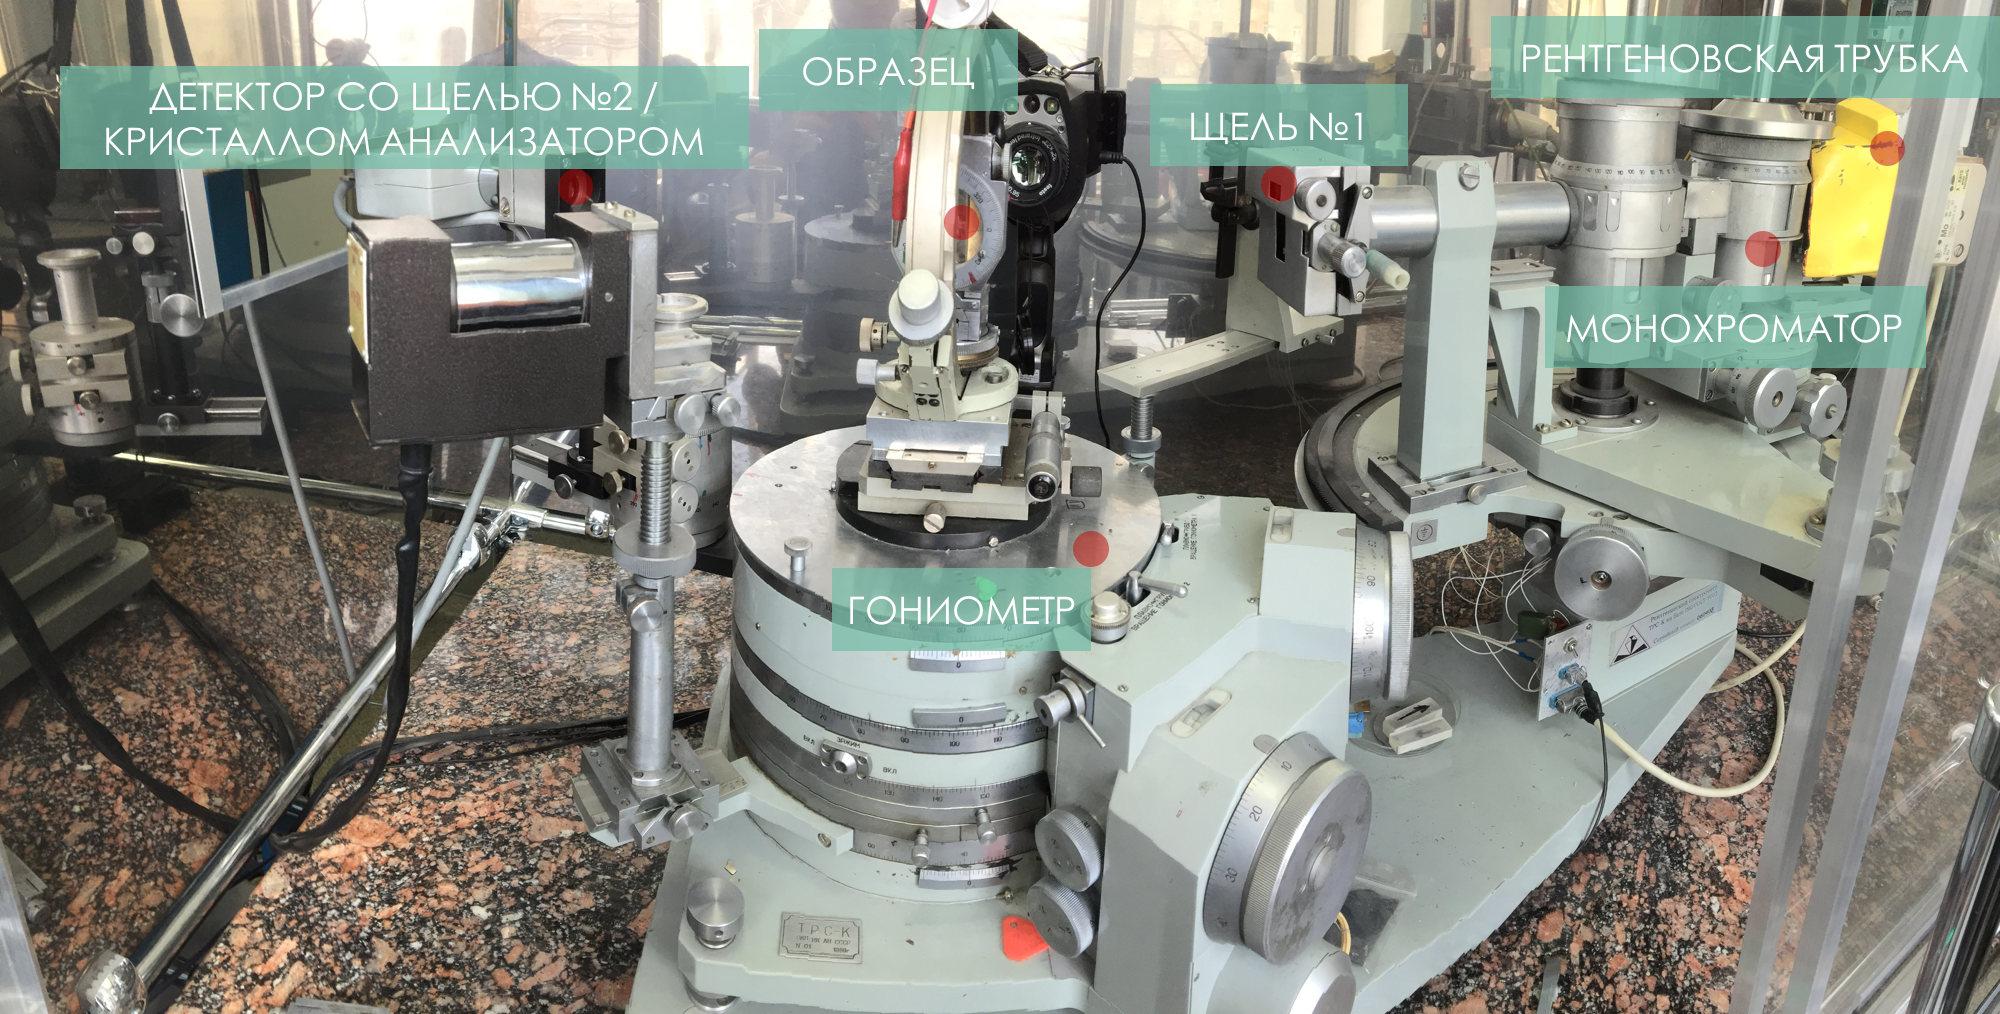
\includegraphics[width=1\textwidth]{images/trs.png}
  \caption{ Трехкристальный рентгеновский спектрометр. Лаборатория рентгеновских
  методов анализа и синхратронного излучения, ФНИЦ "Кристаллография и фотоника"}
  \label{ris:trs}
\end{figure}

ТРС имеет возможность работать в режиме двухкристального эксперимента,
в таком случае непосредственно перед детектором устанавливается щелевое устройство
№ 2, все прошедшие лучи фиксируются детектором.

Для случая необходимости получения трехкристальных кривых дифракционного отражения,
на место перед детектором устанавливается кристалл анализатор, отраженный от анализатора луч
фиксируется детектором.

\subsection{Функция источника}
Спектр рентгеновской трубки является характеристическим, спектральная часть
 которого достаточно хорошо описывается двумя функциями Лоренца взятыми с
 весовыми коэффициентами (\ref{eq:source_spectral}).

 \begin{equation} \label{eq:source_spectral}
   g_{\lambda} (\lambda) = \frac{2\pi}{3}  \left \{ \frac{\delta\lambda_1}{(\lambda - \lambda_1)^2+
   (\delta \lambda_1)^2} + \frac{1}{2} \frac{\delta\lambda_2}{(\lambda-\lambda_1)^2+(\delta\lambda_1)^2} \right \}
  \end{equation}

  Плотность распределения количества потока электромагнитного излучения в зависимости от угла
  отстройки относительно прямолинейного распределения задается функцией Гаусса \ref{eq:source_angle}.

  \begin{equation} \label{eq:source_angle}
    g_{\vartheta} (\vartheta) = \frac{1}{\sigma \sqrt{ 2\pi}} exp  ( -\frac{\vartheta^2}{2\sigma^2} )
   \end{equation}
где $\sigma$ - параметр, который характеризует ширину углового распределения на половине высоты.

\begin{figure}[H]
  \centering
  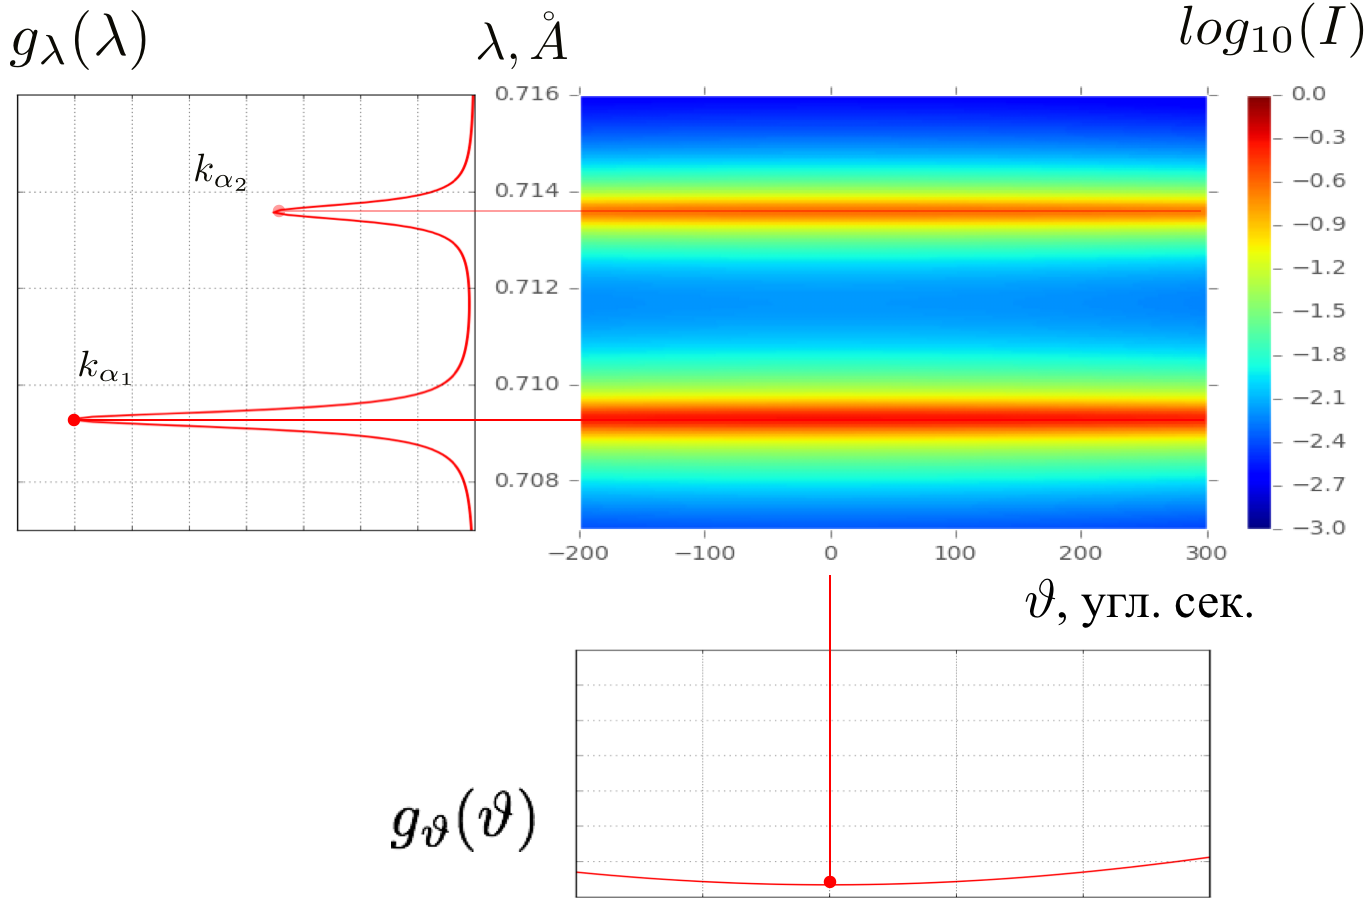
\includegraphics[width=0.6\textwidth]{images/source_distrubition.png}
  \caption{Спектрально – угловое распределение лабораторного источника рентгеновского
   излучения с молибденовым анодом, угловая полуширина распределения составляет $\sigma = 600$ угл. сек. }
  \label{ris:source_distrubition}
\end{figure}


 \subsection{Функция щелевых коллиматоров}
 Рассмотрим преобразование пучка рентгеновского излучения проходящего через систему щелевых коллиматоров.
 \begin{figure}[H]
   \centering
   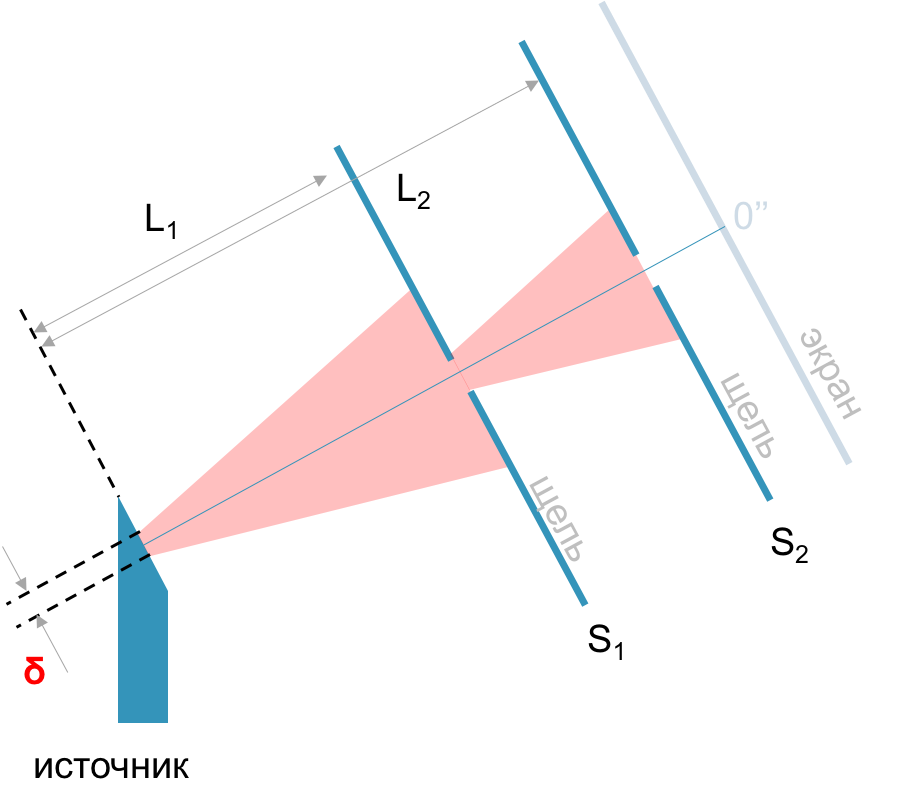
\includegraphics[width=0.6\textwidth]{images/for_slits.png}
   \caption{Схематичное представление щелевых устройств}
   \label{ris:for_slits}
 \end{figure}

На начальном этапе мы рассматривали модель точечного источника излучения.
В таком случае, интенсивность проходящего излучения будет определятся лишь
одним щелевым устройством, которое является более узким в пересчете в угловые
координаты. Далее выберем фиксированные расстояния между элементами,
$L_1 = 570$ мм, $L_2 = 1005$ мм. В случае одинаковых линейных размеров щелей и точечного
источника, интенсивность будет определяться более удаленным щелевым устройством и
распределение интенсивности принимает вид ступеньки (рисунок ~\ref{ris:sourc_map}а). Если источник является
 продолжительным, то угловое распределение интенсивности принимает более сложный вид, как показано на рисунке ~\ref{ris:sourc_map}.

 Для модели точечного источника, интенсивность проходящего излучения будет определять наиболее
 узкой щелью в пересчете на угловые координаты.

 \begin{figure}[H]
   \centering
   \subfloat[Точечный источник]{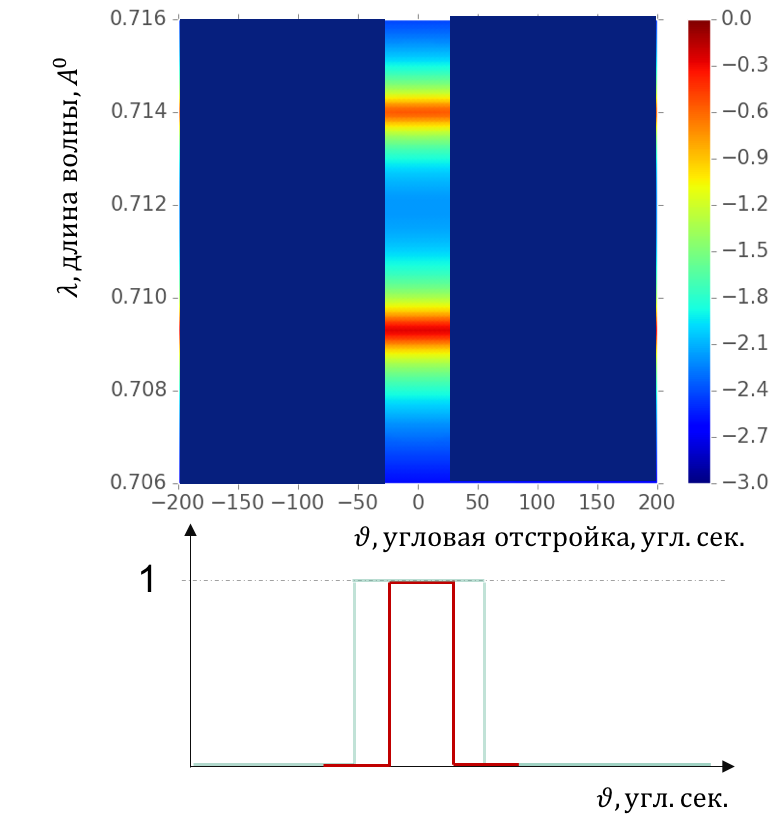
\includegraphics[width=0.45\textwidth]{images/point_sourc_map.png}\label{fig:f1}}
   \hfill
   \subfloat[Источник с линейным размером $\delta = 0.2$ мм]{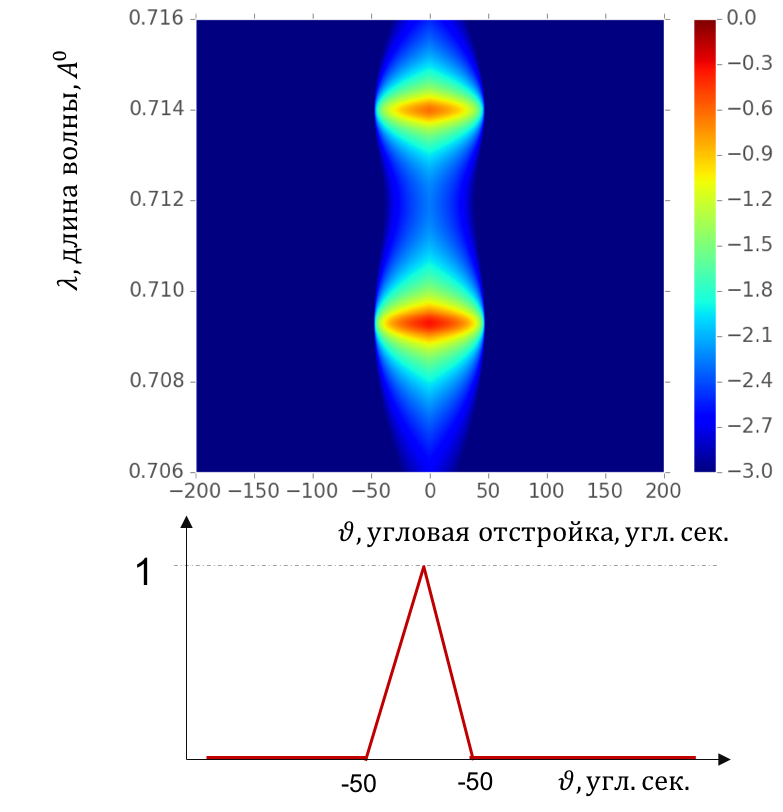
\includegraphics[width=0.45\textwidth]{images/wide_sourc_map.png}\label{fig:f2}}
   \caption{Спектрально угловое распределение источника в система двух щелей}
   \label{ris:sourc_map}
 \end{figure}

   \subsubsection{Дифракция на щели}
      Cowley1979ru на странице 47
  

Измерение кривой дифракционного отражения в двухкристальной схеме представляет
собой измерение зависимости отраженного образцом рентгеновского излучения при
пошаговом повороте исследуемого кристалла относительно падающего на него
излучения в окрестности точного значения угла Брэгга.
Существует несколько схем измерения кривых отражения рентгеновского излучения.

\subsubsection*{$\omega$ - сканирование}
В данном типе сканирования кривая отражения измеряется путем поворота образца
относительно падающего пучка в плоскости дифракции. При таком сканировании
угол между падающим и дифрагированным пучками (угол рассеяния) остается постоянным
(рисунок ~\ref{ris:omega_scan}). Получаемая в результате кривая носит название кривой качания.


\begin{figure}[H]
  \centering
  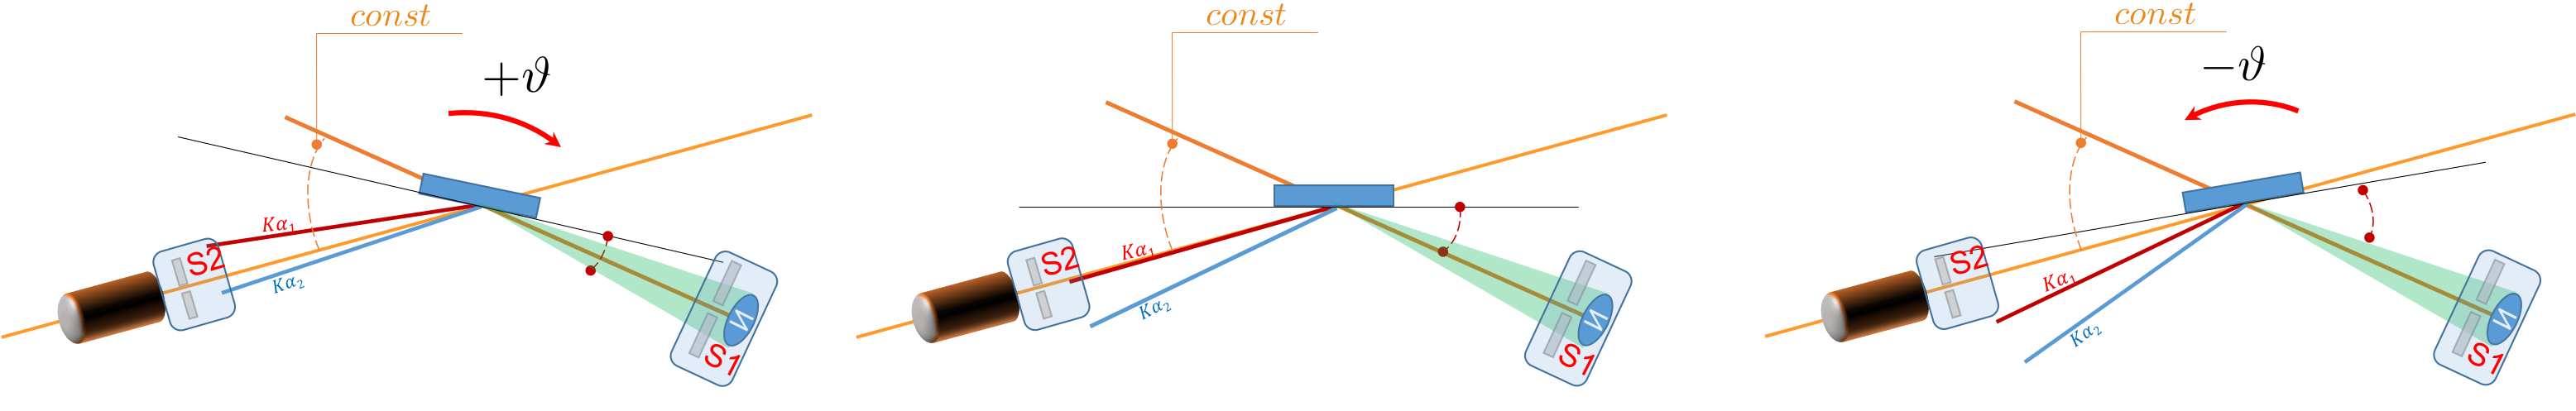
\includegraphics[width=1\textwidth]{images/omega_scan.png}
  \caption{Схема реализации $\omega $ - сканирования}
  \label{ris:omega_scan}
\end{figure}

\subsubsection*{$\vartheta - 2\vartheta$ - сканирование}
В отличие от предыдущего, данный метод сканирования соответствует изменению
 модуля вектора рассеяния при неизменном его угловом положении
 (рисунок ~\ref{ris:theta_2theta_scan}). Угловое положение падающего пучка и
 детектора изменяется синхронно и симметрично относительно используемой системы
 атомных плоскостей, а установленная перед детектором апертурная щель вырезает
  только зеркально отраженную часть пучка. Именно поэтому при построении карт
   пространственного распределения спектра полосы щелей на этих картах остаются
   неподвижными (т.к. несмотря на движение щели  $S_2$ в процессе
    $\vartheta - 2\vartheta$ -  сканирования ее отстройка от зеркального
    положения всегда равна 0).

 \begin{figure}[H]
   \centering
   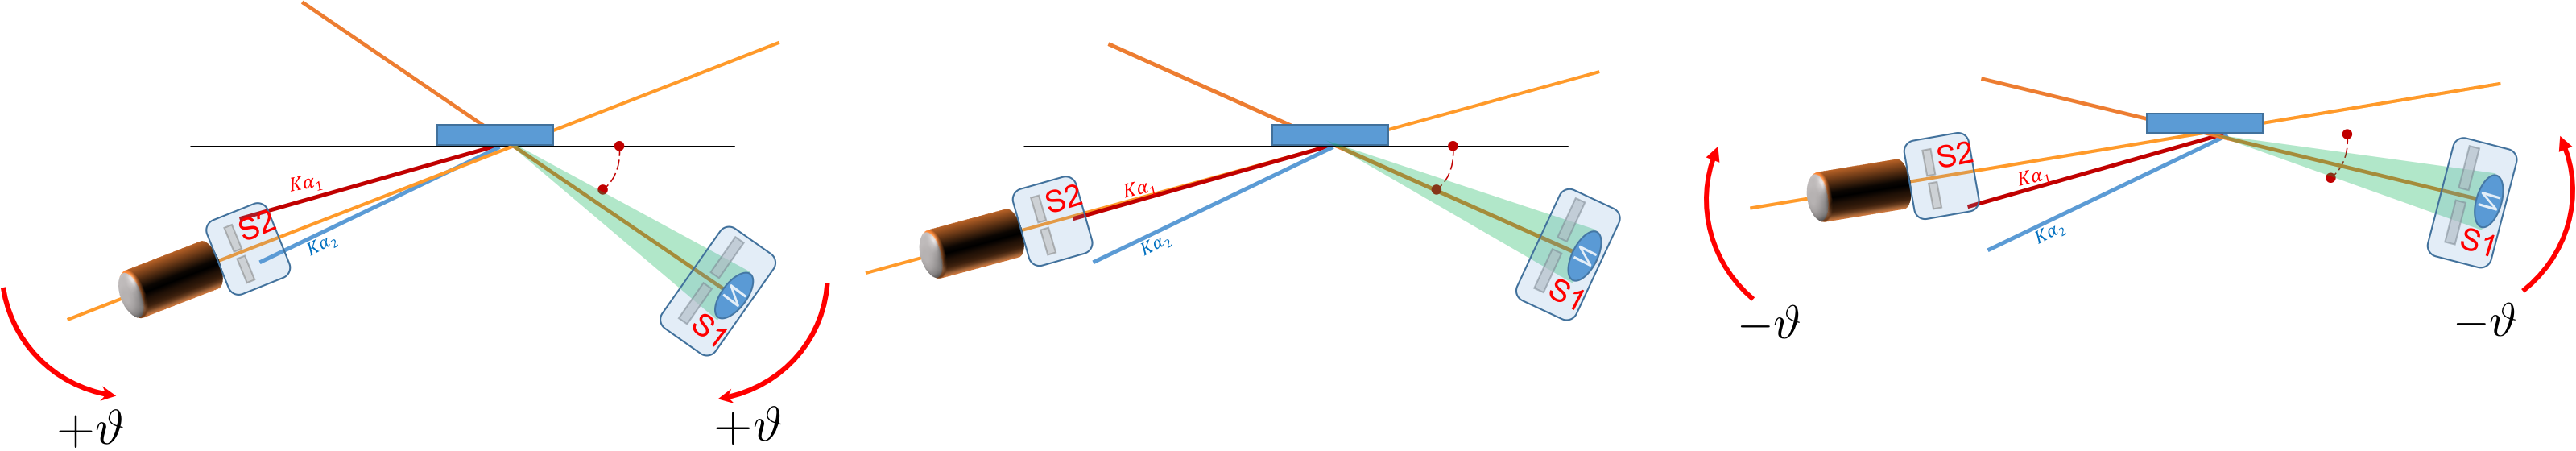
\includegraphics[width=1\textwidth]{images/theta_2theta_scan.png}
   \caption{Схема реализации $\vartheta - 2\vartheta$ - сканирования}
   \label{ris:theta_2theta_scan}
 \end{figure}
Кроме того, используемый подход позволяет наглядно продемонстрировать интересный эффект.
 Независимо от ширины входной и приемной щелей характеристическая линия спектра
 трубки $k_{\alpha 2}$ всегда вносит вклад в КДО, проявляясь в виде дополнительного
 пика на ее хвосте (рис. 2.21). Данный слабый пик возникает за счет того, что
 даже при очень малой входной щели $S_1$ линия $k_{\alpha 2}$ будет, отражаясь на «хвосте»
 кривой монохроматора, пролетать через входную щель и, при определённом угле
 поворота образца, интенсивно дифрагировать в максимуме его собственной кривой
 отражения и давать весомый ($~10^{-6}$) вклад в общую интенсивность КДО.


\subsection{Методика расчета пьзоэлектрических констант по данным дифракции}
